\scanpage{142}
\mspage{70}
une définition directe, \deleted{valable} dans un style encore plus topologique, valable chaque fois au moins (sauf erreur) où on a une immersion locale de \uline{topos}. On va désigner par $\mathcal V_{D',Y}$ le ``voisinage tubulaire'' défini \inserted{en fait} par une immersion \deleted{\unsure{top}} locale topologique. Il a des propriétés de fonctorialité telles, que l'on tire, \deleted{\unsure{dans}} partant d'une situation \deleted{\unsure{de deux}} d'un composé d'immersions locales $D''\mathbin{-}D'\mathbin{-}Y$, \deleted{\unsure{d'un}} un diagramme \unsure{comm.} canonique
\[
(235)\quad\deleted{\unsure{\mathcal V_{D'',Y}}}\quad
\diagram{\begin{tikzcd}[ampersand replacement=\&]
D''\arrow[r,dash]\arrow[d,hook] \& D'\arrow[d,hook] \& \\
\mathcal V_{D'',Y}\arrow[r,"\substack{\mathrm{imm.}\\\mathrm{locale}}"'] \& \mathcal V_{D',Y}\arrow[r,"\substack{\mathrm{imm.}\\\mathrm{locale}}"'] \& Y
\end{tikzcd}}
\]
\margin{\deleted{\unsure{(234)}}
\figure{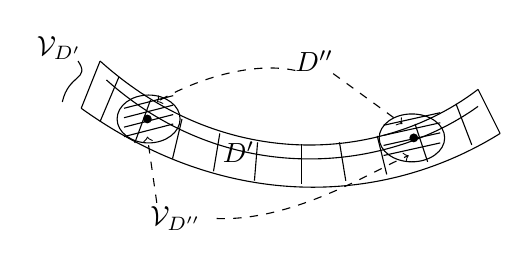
\begin{tikzpicture}[scale=.8]
\draw (-3,1.1) .. controls (-1,-.7) and (1.5,-.5) .. (3,.65);
\draw (-3.3,.35) .. controls (-1,-1.3) and (1.5,-1.2) .. (3.35,-.05);
\draw (-2.9,.8) .. controls (-1,-.9) and (1.5,-.7) .. (3,.38);
\draw (-3,1.1)--(-3.3,.35);\draw (3,.65)--(3.35,-.05);
\draw (-2.7,.85)--(-3,.14);\draw (-2.2,.48)--(-2.45,-.2);
\draw (-1.7,.18)--(-1.85,-.45);\draw (-1.1,-.05)--(-1.2,-.65);
\draw (-.5,-.19)--(-.55,-.8);\draw (.2,-.22)--(.2,-.85);
\draw (.8,-.19)--(.9,-.8);\draw (1.4,-.09)--(1.55,-.7);
\draw (2,.1)--(2.2,-.5);\draw (2.65,.42)--(2.9,-.23);
\draw (-2.23,.18) ellipse (.5 and .38);\draw (1.95,-.12) ellipse (.52 and .38);
\foreach \y in {-.1,.05,.2,.35} {\draw (-2.62,\y)--(-1.84,\y+.2);}
\foreach \y in {-.4,-.24,-.08,.08} {\draw (1.5,\y)--(2.4,\y+.2);}
\fill (-2.25,.18) circle(2pt);\fill (1.98,-.12) circle(2pt);
\node at (-.8,-.35) {$D'$};\node at (.4,1.1) {$D''$};
\draw[->,dashed] (.1,.95).. controls (-.6,1.1) and (-1.5,.8)..(-2.1,.45);
\draw[->,dashed] (.7,.9)--(1.8,.1);
\node at (-3.65,1.3) {$\mathcal V_{D'}$};\draw (-3.35,1.1) .. controls (-3.15,.8) and (-3.5,.9)..(-3.6,.45);
\node at (-1.8,-1.4) {$\mathcal V_{D''}$};
\draw[dashed,->] (-2.1,-1.15)--(-2.25,-.1);
\draw[dashed,->] (-1.15,-1.4).. controls (.1,-1.45) and (1.4,-.6)..(1.9,-.4);
\end{tikzpicture}}}

\deleted{\unsure{Donc}} Pour l'instant, on n'a pas utilisé le diviseur $\Theta$ à croisements normaux dans $Y$ définissant \inserted{l'ouvert} $Y^{*}=Y\setminus\Theta$. \unsure{Nou|N.} Nous considérons maintenant l'image inverse de $Y^{*}$ dans $\mathcal V_{D',Y}$ et $\mathcal V_{D'',Y}$, soient $\mathcal V^{*}_{D',Y}$ et $\mathcal V^{*}_{D'',Y}$, s'insérant dans un diagramme
\margin{141}
